\chapter{Solution Details}
\label{cha:solution_details}

The proposed simulation framework is implemented in a small proof of concept application. The application provides a simple playground to test, evaluate and demo various scenes. The provided application was only developed and tested under MacOS X Lion, but the small number of required dependencies are all available as cross-platform libraries for Windows, MacOS X and Linux. 

The application was written in the C++ programming language because it is the predominate language in the area of physical simulations and for the easy integration with dependencies. The graphics pipeline runs on OpenGL and to simplify its usage the OpenGL Utility Toolkit (GLUT) was also heavily used. The only other major dependency is the Bullet Physics Library (Bullet).

Bullet is almost exclusively used to handle and manage the rigid bodies in the scene. This includes integrating velocities and positions as well as handling collision detection for rigid-to-rigid collisions. Collision resolution is done manually and partially shared with particle-to-rigid collisions. Bullet is not used deliberately for the collision detection and responses between rigid bodies and oriented particles. Both the external collisions as well as the inner force propagations are implemented in their respective collision handlers. This allows for the necessary customizations to implement the proposed algorithms.

Bullet's built in linear math module is used throughout the code for the various mathematical formulas and provides the basic vector and matrix primitives. This includes all the code required to implement the deformable parts of the simulation. Every oriented particle, their simulation and their collisions are calculated using the provided math functions. However, apart from these functions the code for the oriented particles and custom collision handlers is completely hand-written. This is also the reason why the performance of these code sections is not ideal. The focus of the current implementation is solely a proof of concept and only meant to allow for general and simple comparisons.

\section{Code Structure}

The complete implementation requires only four classes. The main application function only sets up the graphics context including the ability to navigate the scene with the keyboard and runs the main execution loop for the simulation.

\paragraph{Simulation Class}
The Simulation class implements everything required for setting up the concrete scene and handles each simulation step. The simulation class also implements all collision code. The collisions between purely rigid bodies are handed off to bullet for detection and the resolution is then manually calculated inside the simulation class. For oriented particles the code for the collision detection and resolution is entirely implemented inside the class itself in order to provide maximum customization.

Currently the scenes always consist of a ground and a variably sized block, which will be the object to be picked up. The ground is a simple static rigid body and does not move or react to forces during the entire simulation. The block is also a rigid body but it is completely alive. This means both gravity and later the pickup forces act and modify the state of the block. The block can have both an arbitrary size and mass.

To either side of the block two fingers are positioned. These fingers can either be completely rigid or be the new combined bodies consisting of both a rigid inner bone and a soft outer tissue. If the fingers are rigid they are simulated in exactly the same way as any other rigid body with the help of the bullet library. Combined bodies are simulated using the custom CombinedBody class which will be described later.

For simulation purposes the force and resulting velocities are set manually for the two fingers, regardless if they are rigid bodies or combined bodies. This is done to simulate fixed fingers which cannot be pushed apart and exert a constant push force as well as a constant force upwards. In order to facilitate this property the linear velocity in x is capped at zero for both pushing directions, this means the left finger is only allowed to push into the positive direction and has a minimum velocity in x of zero. The right finger correspondingly is only allowed to push into the negative direction and has a minimum maximum velocity of zero. In velocity in y is not capped as it will always point upwards, however both fingers velocity in y is synchronized so that one finger can't move faster than the other. The velocity in z as well as the angular velocity is always set to zero so no movement can occur. These modifications are necessary for the current simple simulation only, in an improved version controllers and motors would be needed to more realistically model fixed and stable fingers.

\paragraph{CombinedBody Class}
The CombinedBody class holds all the information required for the proposed two part body consisting of an inner rigid bone and outer soft tissue. The rigid part is built using the btRigidBody class provided by the bullet library. For the deformable part multiple instances of the custom class ParticleGroup is maintained. The CombinedBody class handles the states for the rigid body and all particles and provides basic functions to apply forces and integrate the velocities and positions.

One major functionality integrated into the CombinedBody class is the initialization of the soft outer tissue. Also the structure of the oriented particles in the tissue is arbitrary, as far as the simulation is concerned a concrete sample implementation is provided. The underlying geometric structure chosen relies on an evenly distributed number of so called attached particles across the surface of the inner rigid body. Currently only a version for box-like shaped bodies is provided. The layout algorithm for the attached particles starts by iterating over all faces of the box. An attached particle is added for each corner. Then depending on a customizable density parameter additional particles are added to each edge. Finally the rest of the face is filled according to the grid defined by the particles on the corners and edges. An illustration of this can be seen in figure \ref{fig:combined_body_density}.

\begin{figure}[htb]
  \centering
  \subfigure[$density = 1$]{
      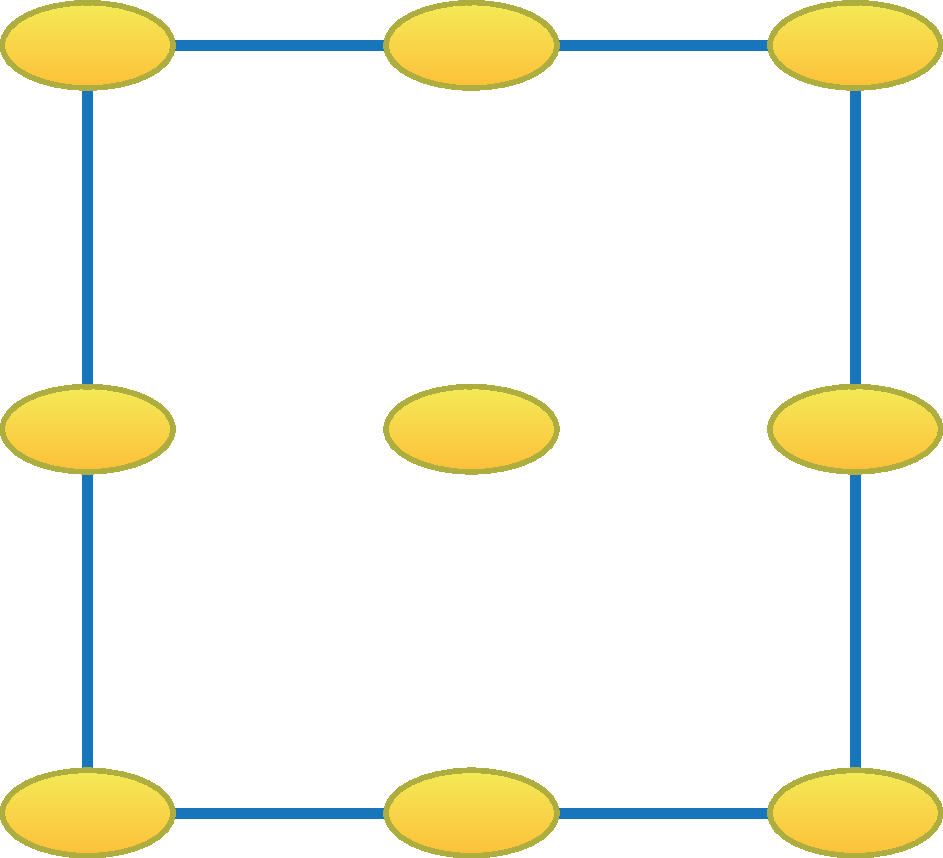
\includegraphics[width=.35\textwidth]{images/combined_body_density_1.pdf}
     \label{subfig:combined_body_density_1}
  }
\hspace{2cm}
  \subfigure[$density = 2$]{
      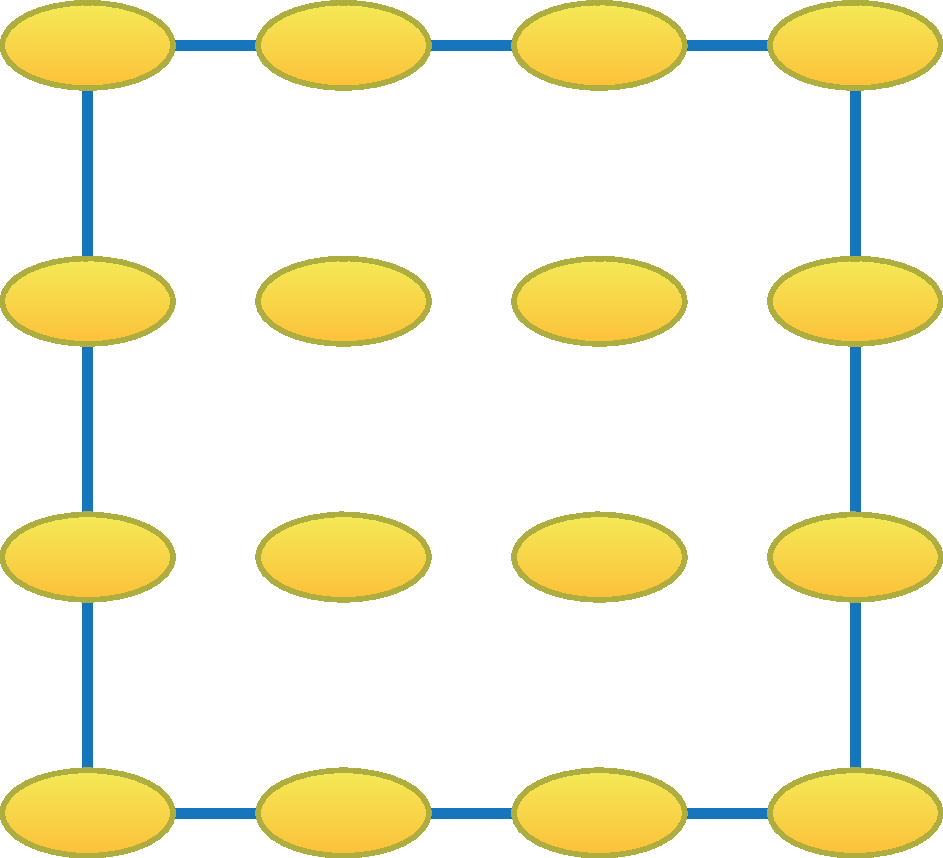
\includegraphics[width=.35\textwidth]{images/combined_body_density_2.pdf}
     \label{subfig:combined_body_density_2}
  }
  \caption{Tissue particle density}
  \label{fig:combined_body_density}
\end{figure}

For the outer soft tissue the inner attached particles are simply extruded by a configurable factor from the center of mass of the inner core. This results in a simple one layer outer layer. Again the simulation itself does not place any restrictions on the structure of the tissue, but this simple algorithm has proved to be sufficient. The last step required for a complete model of the deformable outer part is generating the implicit particle groups required for shape matching.

The concrete algorithm to accomplish this is not really important, only two restrictions have to be taken care of. First a high enough degree of interconnectiveness must be ensured. In the original oriented particles paper the implicit connection is simply taken from the underlying mesh of vertices connected by the edges. The second restriction is that the outer particles have to be connected to the attached particles on the surface, as otherwise the skin would just come off.

The current implementation iterates over all particles on each respective layer (attached and outer). For each particle $p$ a list of all particles in the current layer is generated and sorted by the distance to particle $p$. This ensures that the particle itself is always at index $0$ of this list, followed by its closest neighbors. A configurable number $n = groupSize$ of particles taken from the beginning of this list is then added to a particle group with the particle $p$ at the center. Lastly the corresponding particle in the other layer is also added with the help of the extrude factor, ensuring the connection of both layers. So every group in the end consists of $n = groupSize + 1$ particles. This is done for both the attached particle layer, as well as the outer particle layer in order to generate all the particle groups required for shape matching.

\paragraph{ParticleGroup Class}
The ParticleGroup class holds all particles belonging to a specific implicit shape matching group. It implements all the functionality required to execute the shape matching algorithm. This includes calculating the current center of mass and the moment matrix across all particles. The polar decomposition is also implemented here. The implementation adapted from Higham \cite{Higham:1986vx} as it is implemented in the bullet library\footnote{\text{http://bulletphysics.com/Bullet/BulletFull/btSoftBodyInternals\_8h\_source.html}}. Using all these subcomponents in the final calculation of the goal positions and subsequent adjustment of the predicted position is also the responsibility of the particle group.

\paragraph{Particle Class}
The Particle class holds all the required state variables for an oriented particle as described in section \ref{sec:oriented_particles}. This also includes all derived and intermediary variables. Both the predicted position and orientation of the particle are maintained here as well as the current moment matrix for a single particle.

\section{Loop}

This section illustrates the simulation step executed for each time step. It only shows the loop as it is implemented for the deformable scenario. The scenario with only rigid bodies is essentially identical to the sample loop provided in section \ref{sec:rigid_body_simulations} about rigid body simulations.

\begin{algorithm}[htb!]
\caption{Combined Body Simulation Loop}
\begin{algorithmic}[1]
\FORALL{bodies $b_{all}$}
	\STATE{apply gravity}
	\STATE{integrate velocity}
	\STATE{predict state}
\ENDFOR
\FORALL{fingers $f$}
	\FORALL{outer particles $p_{outer}$}
		\STATE{resolve collision with ground}
	\ENDFOR
	\FORALL{outer particles $p_{outer}$}
		\STATE{resolve collision with block}	
	\ENDFOR
\ENDFOR
\FORALL{gauss-seidel iterations $i$}
	\FORALL{fingers $f$}
		\FORALL{particle groups $g$}
			\STATE{do shape matching}
		\ENDFOR
	\ENDFOR
\ENDFOR
\FORALL{fingers $f$}
	\FORALL{attached particles $p_{attached}$}
		\STATE{apply impulse to bone}
		\STATE{snap to bone}
	\ENDFOR
\ENDFOR
\FORALL{rigid bodies $b_{rigid}$}
	\STATE{resolve collisions}
\ENDFOR

\FORALL{bodies $b_{all}$}
	\STATE{integrate forward}
\ENDFOR
\end{algorithmic}
\end{algorithm}

The first step of the loop applies all external forces to all bodies in the simulated world. For the particle in the tissue layer of the combined bodies this directly modifies the velocity of each particle. The velocities of the inner rigid body and all other rigid bodies in the scene are then integrated separately using the provided functions from bullet. After that the position and orientation of all bodies and particles are predicted so that potential collisions can be resolved.

The different types of collisions are all detected and resolved separately. First all outer particles are checked against the ground and if necessary their respective predicted state adjusted. After that follows the collision resolution with the block in between the two fingers. This step not only modifies and redefines the predicted state of the outer particles but potentially also applies the required impulses to the rigid body of the block, including both the normal forces as well as the forces caused by friction.

Having adjusted the predicted state for all outer particles due to potential collisions the algorithm now starts with the Gauss-Seidel iterations. The concrete iteration count is set to low single digit number, which seems to provide a good balance between performance and robustness. For each iterations all shape matching groups are updated and the particles partially moved to their calculated goal positions. These updates affect all particles, both outer particles but also attached particles. This step is identical to the way shape matching is implemented in the original oriented particles paper \cite{Muller:2011gn}.

After the final predicted positions for all particles the attached particles are realigned with their true position on the surface of the bone. This process also propagates the impulses caused by the moving tissue onto the inner rigid body. After the required impulse has been calculated and applied all attached particles are snapped back to their position on the surface.

The next step simply resolves all potential collisions between purely rigid bodies in the world. These bodies might potentially include the velocities they received from the collision with oriented particles. The final step in the loop then integrates all bodies and particles forward in time, updating both the positions and orientations of everything according to the modifications caused by the intermediary collisions and shape matching. This new state is then used in the next time step to rerun the loop form the beginning.